\documentclass{article}
\usepackage{graphicx}
\usepackage{authblk}
\usepackage{amsmath}
\usepackage{listings}

\begin{document}


\title{THEORETICAL NEUROSCIENCE II \\ EXERCISE 06 - RESCOLA-WAGNER RULE}
\date{05 June 2013}
\author[1]{Yunus Emre Demiray, Taygun C. Uzuneser, \c{S}eyma Bayrak\thanks{seyma.bayrak@st.ovgu.de}}
\affil[1]{\footnotesize  Otto von Guericke University of Magdeburg}
\maketitle

\newpage

\section{Steady State Condition}
Rescola-Wagner rule defines the weight evolution as the following:
\begin{equation}
 \textbf{w}^{i+1}=\textbf{w}^{i}+\epsilon \delta_i \textbf{u}^i
\end{equation}
where $\epsilon$ is the learning rate, and $\delta$ is the prediction error which is the difference between the actual reward $r$ and the expected reward $v$, such that $\delta=r-v$.

Steady state condition can be applied by assuming no change in wieghts, simply $\textbf{w}^{i+1}-\textbf{w}^{i}=0$. Let us call the weight at the steady state point as $\textbf{w}_{ss}$, and derive it from $\langle \delta \textbf{u} \rangle$
\begin{equation*}
 \langle \delta \textbf{u }\rangle=  \langle R\textbf{u} - v\textbf{u} \rangle =\langle R\textbf{u} \rangle - \langle \textbf{w}.\textbf{uu}  \rangle = 0 \longrightarrow \textbf{w}.\langle  \textbf{uu} \rangle=\langle R\textbf{u} \rangle \longrightarrow \textbf{w}=\frac{\langle R\textbf{u} \rangle}{\langle \textbf{uu} \rangle}
\end{equation*}
Introduce the correlation matrix $\textbf{Q}=\langle \textbf{uu} \rangle$, then
\begin{equation}
 \textbf{w}_{ss}=\textbf{Q}^{-1}.\langle R\textbf{u} \rangle
\end{equation}

\section{Expected Values and Correlations}
Two binary stimuli from (e.g. like from both eyes, I prefer to use Right and Left notation not to be confused while calculating) and their probabilities are defined as the following;
\begin{equation*}
u_{R,L} \;\; \epsilon \;\;\{0,1\} \ \;\;meaning \;\; \textbf{u} \epsilon \{ \left ( \begin{array}{cc} 1 \\ 1  \end{array} \right ) \ , \left ( \begin{array}{cc} 1 \\ 0  \end{array} \right ) \ , \left ( \begin{array}{cc} 0 \\ 1  \end{array} \right ) \ , \left ( \begin{array}{cc} 0 \\ 0  \end{array} \right ) \ \}
\end{equation*}
that occurs with probabilities
\begin{equation*}
 p_{11}, \; p_{00}, \; p_{01}, \;p_{10} ;\;\;\;\;\;\;\;\;\; \longrightarrow  \;\;\;\;\;\;\;\;\;\; p_{11}+p_{00}+p_{01}+p_{10}=1
\end{equation*}
The exercise assumes an equally binary reward, which has ben already given above, $R$, that is alo either 1 or 0. However, how frequent the stimuli is rewarded also defined probabilistically. If we denote the probability of being rewarded as $r_{xy}$, that means for the probability of reward when the first stimulus is $x$ and the second is $y$. Let us write all the possible rewards corresponding to our stimulus \textbf{u}:
\begin{equation*}
  0 \leq r_{11}, \; r_{00}, \; r_{01}, \;r_{10} \leq 1
\end{equation*}

Derivation of the expected stimuli:
\begin{equation*}
 \langle u_R  \rangle =\sum_{u_{R,L} \; \epsilon\{0,1\}} p_{RL}.u_R=p_{00}.0+p_{01}.0+p_{11}.1+p_{10}.1=p_{11}+p_{10}
\end{equation*}
\begin{equation*}
 \langle u_L  \rangle =\sum_{u_{R,L} \; \epsilon\{0,1\}} p_{RL}.u_L=p_{00}.0+p_{01}.1+p_{11}.1+p_{10}.0=p_{11}+p_{10}
\end{equation*}

\begin{equation}
 \langle \textbf{u}\rangle = \left ( \begin{array}{cc} \langle u_R \rangle \\ \langle u_L\rangle  \end{array} \right ) \ = \left ( \begin{array}{cc}  p_{11}+p_{10}  \\  p_{11}+p_{10}  \end{array} \right ) \
\end{equation}

Derivation of correlation matrix of the stimulus vector:
\begin{equation*}
 \textbf{Q}=\langle \textbf{uu} \rangle = \langle \textbf{u}.\textbf{u}^T \rangle = \langle \left ( \begin{array}{cc}  u_R  \\ \ u_L  \end{array} \right ). \left ( \begin{array}{cc}  u_R   \ u_L  \end{array} \right )  \rangle =\left ( \begin{array}{cc} \langle u_R u_R \rangle & \langle u_R u_L \rangle \\ \langle u_Lu_R\rangle &  \langle u_L u_L \rangle \end{array} \right )
\end{equation*} 
\begin{equation*}
 \langle u_R  \rangle =\sum_{u_{R,L} \; \epsilon\{0,1\}} p_{RL}.(u_R)^2=p_{00}.0^2+p_{01}.0^2+p_{11}.1^2+p_{10}.1^2=p_{11}+p_{10}
\end{equation*}
\begin{equation*}
 \langle u_L  \rangle =\sum_{u_{R,L} \; \epsilon\{0,1\}} p_{RL}.(u_L)^2=p_{00}.0^2+p_{01}.1^2+p_{11}.1^2+p_{10}.0^2=p_{11}+p_{01}
\end{equation*}
\begin{equation*}
 \langle u_R u_L \rangle =\sum_{u_{R,L} \; \epsilon\{0,1\}} p_{RL}.u_Ru_L=p_{00}.0.0+p_{01}.0.1+p_{11}.1.1+p_{10}.1.0=p_{11}
\end{equation*}
\begin{equation*}
 \langle u_R u_L \rangle =\langle u_L u_R \rangle
\end{equation*}
\begin{equation}
 \textbf{Q}=\langle \textbf{uu} \rangle = \left ( \begin{array}{cc}  p_{11}+p_{10}  & p_{11} \\ p_{11}+p_{01}  & p_{11}+p_{01} \end{array} \right )
\end{equation} 
Derivation of the expected value of the reward-weighted stimuli $\langle r \textbf{u } \rangle$:
\begin{equation*}
 \langle r u_R \rangle =\sum_{u_{R,L} \; \epsilon\{0,1\}} p_{RL}.r_{RL}.u_R=p_{00}.r_{00}.0+p_{01}.r_{01}.0+p_{11}.r_{11}.1+p_{10}.r_{10}.1
\end{equation*}
\begin{equation*}
=p_{11}.r_{11}+p_{10}.r_{10}
\end{equation*}
\begin{equation*}
 \langle r u_L \rangle =\sum_{u_{R,L} \; \epsilon\{0,1\}} p_{RL}.r_{RL}.u_L=p_{00}.r_{00}.0+p_{01}.r_{01}.1+p_{11}.r_{11}.1+p_{10}.r_{10}.0 
\end{equation*}
\begin{equation*}
=p_{11}.r_{11}+p_{01}.r_{01}
\end{equation*}
\begin{equation}
 \langle r \textbf{u} \rangle= \left ( \begin{array}{cc}  p_{11}.r_{11}+p_{10}.r_{10} \\ p_{11}.r_{11}+p_{01}.r_{01} \end{array} \right )
\end{equation} 
\section{Independent Conditioning}
We now consider a situation in which two stimuli are conditioned independently. The assigned probabilities for the stimuli input and rewards are stated below. 
\begin{equation*}
 p_{01}=p_{10}=\frac{1}{}, \;\;\;\; p_{11}=p_{00}=0, \;\;\;\;r_{10}=1, \;\;\;\;r_{01}=\frac{3}{4}, \;\;\;\; r_{11}=r_{00}=0
\end{equation*}
As seen above, two stimuli are not allowed to happen (being 1) together. 

Derive the $\textbf{w}_{ss}$ just by inserting the given probability values into Equations 5,4,2: 

\begin{equation*}
\textbf{Q}^{-1}= \left ( \begin{array}{cc}  1/2 & 0 \\ \ 0 & 1/2  \end{array} \right )^{-1}=\left ( \begin{array}{cc}  2 & 0 \\ \ 0 & 2  \end{array} \right )  \;\;\;\;\; and \;\;\;\;\; \langle r \textbf{u} \rangle= \left ( \begin{array}{cc}  1/2  \\ \ 3/8 &  \end{array} \right )
\end{equation*}

\begin{equation*}
\textbf{w}_{ss}= \textbf{Q}^{-1}.\langle R\textbf{u} \rangle= \left ( \begin{array}{cc}  2 & 0 \\ \ 0 & 2  \end{array} \right ) . \left ( \begin{array}{cc}  1/2  \\ \ 3/8 &  \end{array} \right )=\left ( \begin{array}{cc}  1 \\ \ 3/4   \end{array} \right ) 
\end{equation*}

A sequence of $N=200$ stimuli and rewards by implementing the Rescola-Wagner Rule are created by the provided MATLAB scripts $\textbf{eidep}\_\textbf{condit.m}$ and \textbf{ShowSequence.m}. The learning rate was assigned as $\epsilon=0.1$. The following figure is eliminated. 


\begin{center}
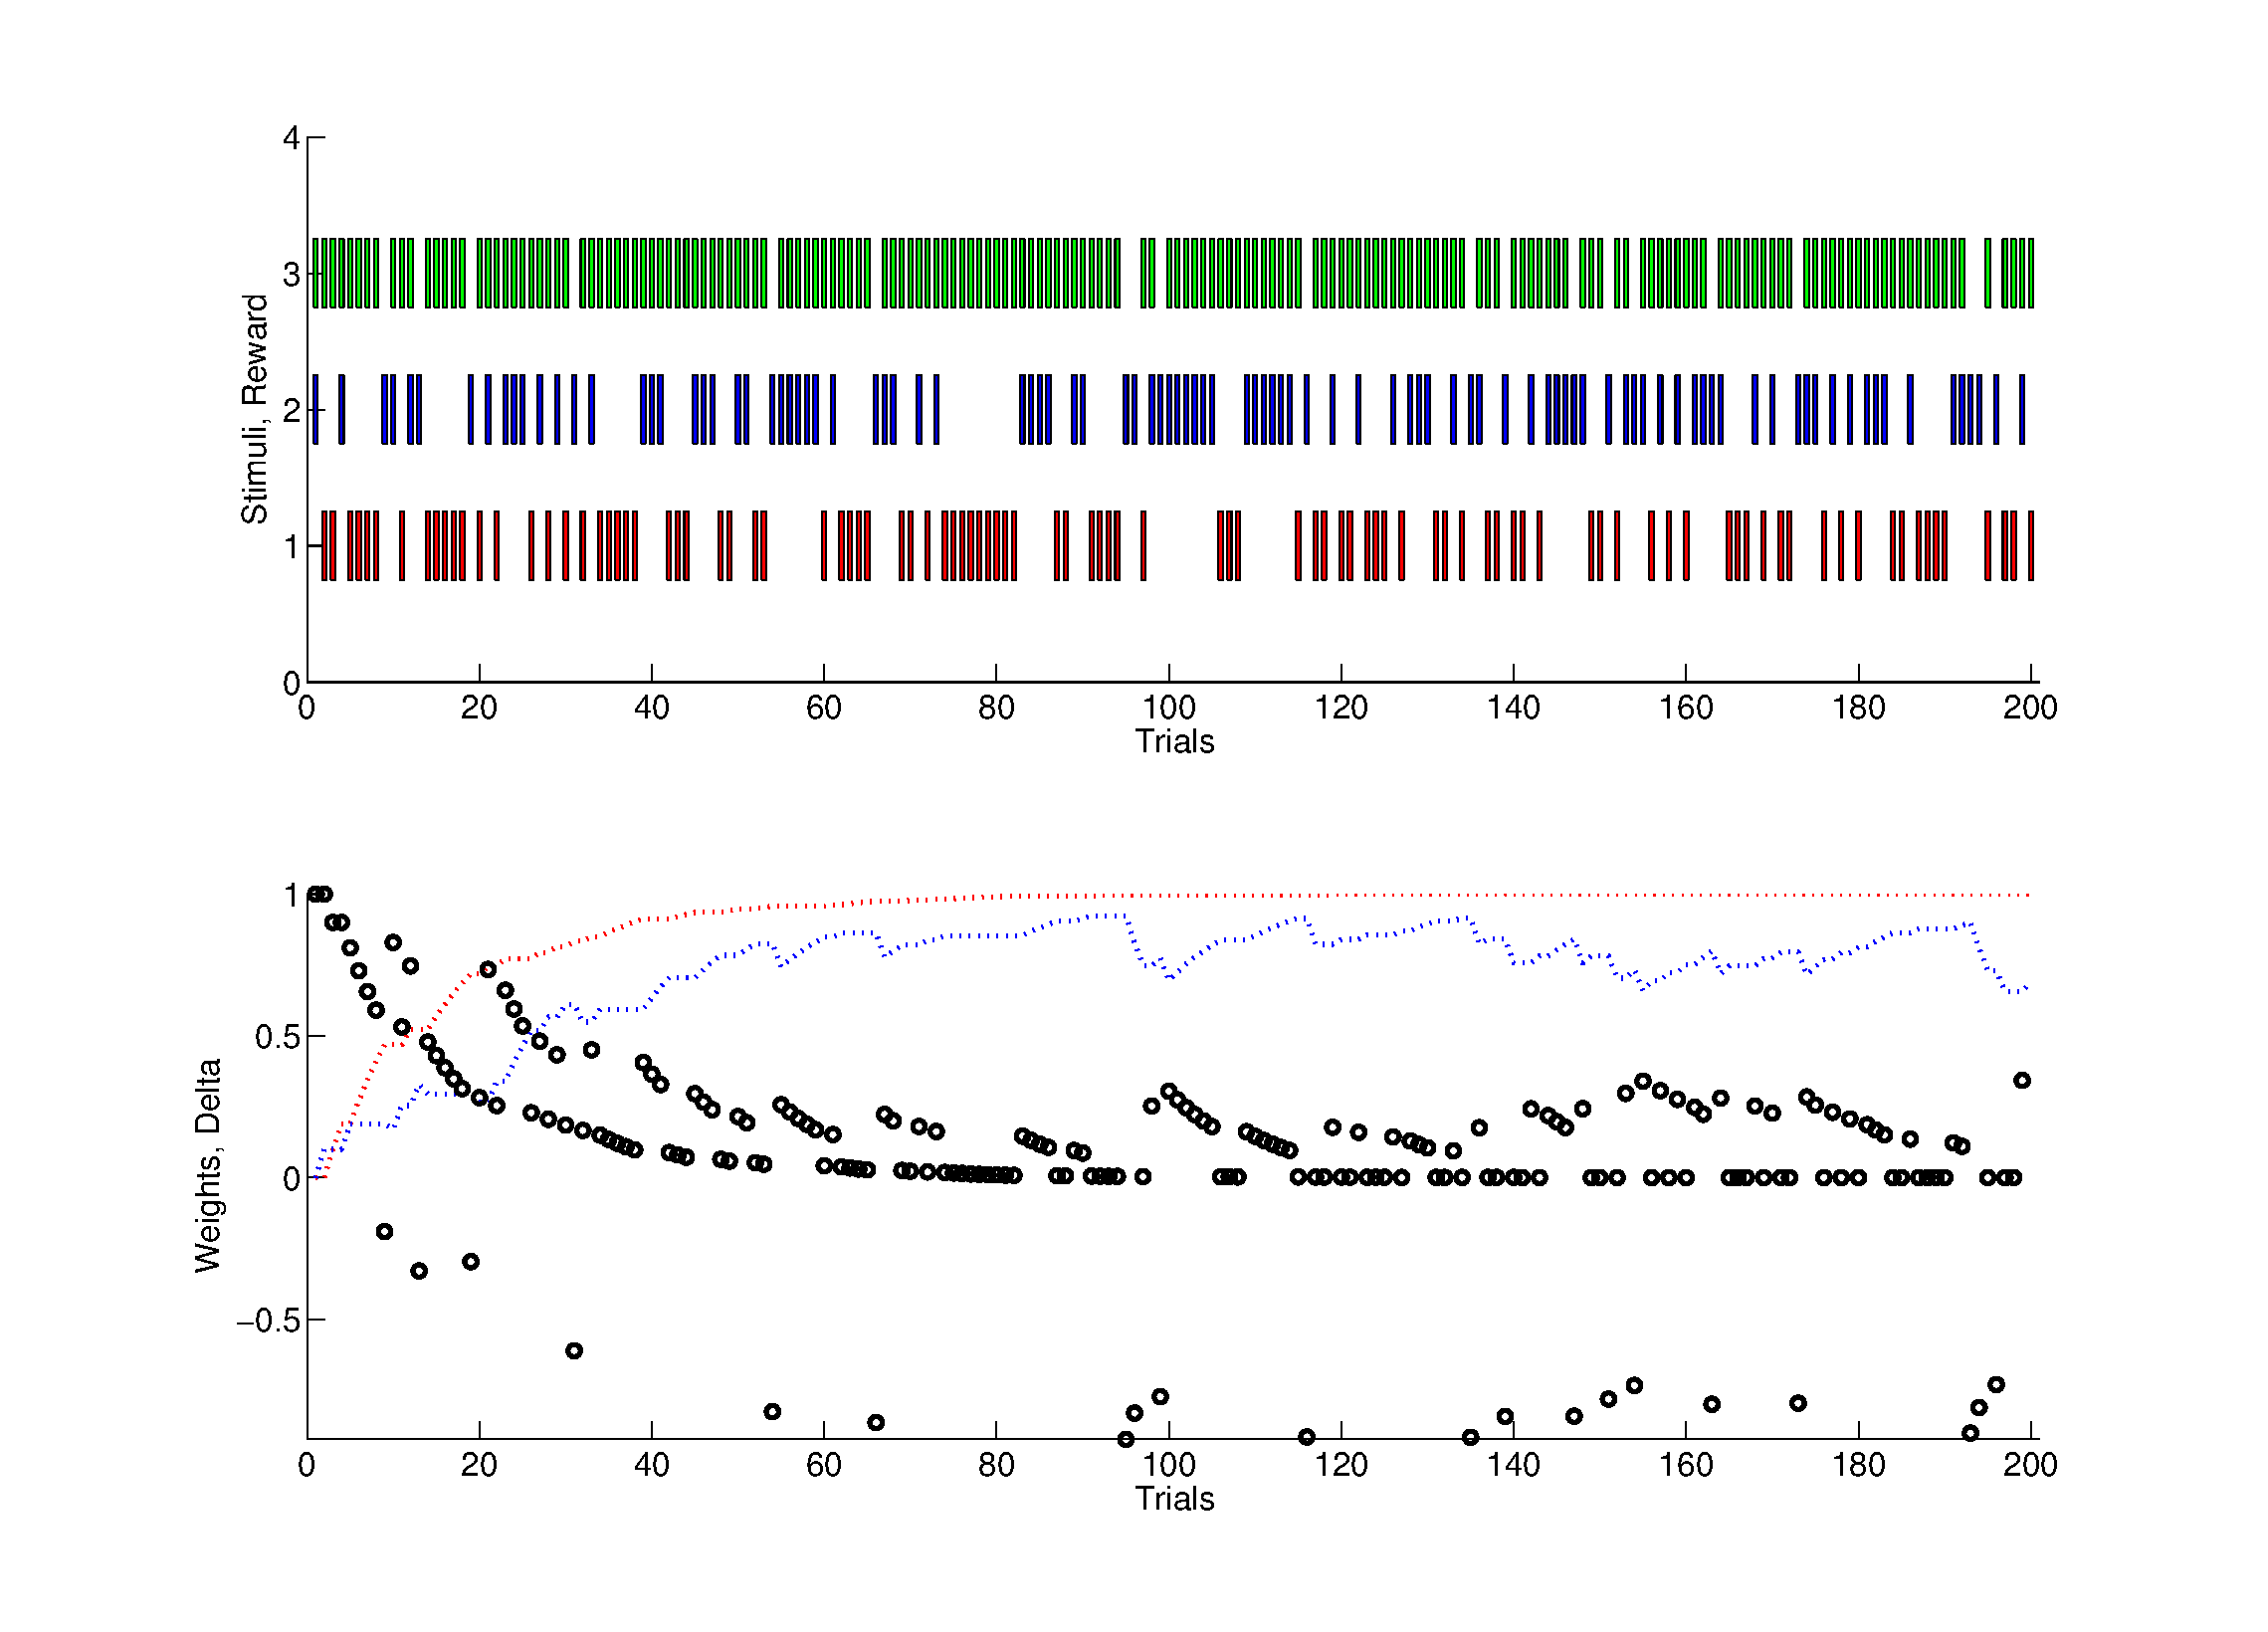
\includegraphics[width=\textwidth]{indep.eps}
% tau4_M1.eps: 0x0 pixel, 300dpi, 0.00x0.00 cm, bb= -304   -42   918   834
\begin{footnotesize}
 Figure 1, upper graph: green and blue bars represent stimuli distribution in N=200 trials, greens are for $u_R$ and blues are for $u_L$. The red bars stand for the corresponding rewards. Lower graph: red and blue dotted lines represent the weight evolution, black circles stand for the $\delta$ values for the corresponding weight evolutions.
\end{footnotesize}
\end{center}


\subsection{Discussion}
\begin{itemize}
\item Rewards are assigned to particular stimuli with Rescola-Wagner Rule. For each stimulus, a conditional reward expectation is learned. 
 \item Weights converge to the steady state values stated as $w_{ss}$, as it is seen the red dotted line converges to 1, and blue dotted line converges to 3/4. We can even say weights converge to expected reward.
\item The prediction error $\delta$ for both of the weight evolutions converge to 0. At steady state the average prediction error vanishes. This represents the learning. The negative values of $\delta$ might represent the failure of an expected reward.
\end{itemize}

\section{Inhibitory Conditioning}
Consider a situation in which one stimulus is rewarded only when it occurs alone. That causes the inhibitory conditioning, the probabilities are given below.
\begin{equation*}
 p_{11}=p_{10}=1/2, \;\;\; p_{01}=p_{00}=0,\;\;\;r_{11}=r_{00}=r_{01}=0, \;\;\; r_{10}=3/4
\end{equation*}
Derivation of the steady state weights:
\begin{equation*}
\textbf{Q}^{-1}= \left ( \begin{array}{cc}  1 & 1/2 \\ \ 1/2 & 1/2  \end{array} \right )^{-1}=\left ( \begin{array}{cc}  2 & -2 \\ \ -2 & 4  \end{array} \right )  \;\;\;\;\; and \;\;\;\;\; \langle r \textbf{u} \rangle= \left ( \begin{array}{cc}  3/8  \\ \ 0 &  \end{array} \right )
\end{equation*}
\begin{equation*}
\textbf{w}_{ss}= \textbf{Q}^{-1}.\langle R\textbf{u} \rangle= \left ( \begin{array}{cc}  2 & -2 \\ \ -2 & 4  \end{array} \right ) . \left ( \begin{array}{cc}  3/8  \\ \ 0 &  \end{array} \right )=\left ( \begin{array}{cc}  3/4 \\ -3/4   \end{array} \right ) 
\end{equation*}
\begin{center}
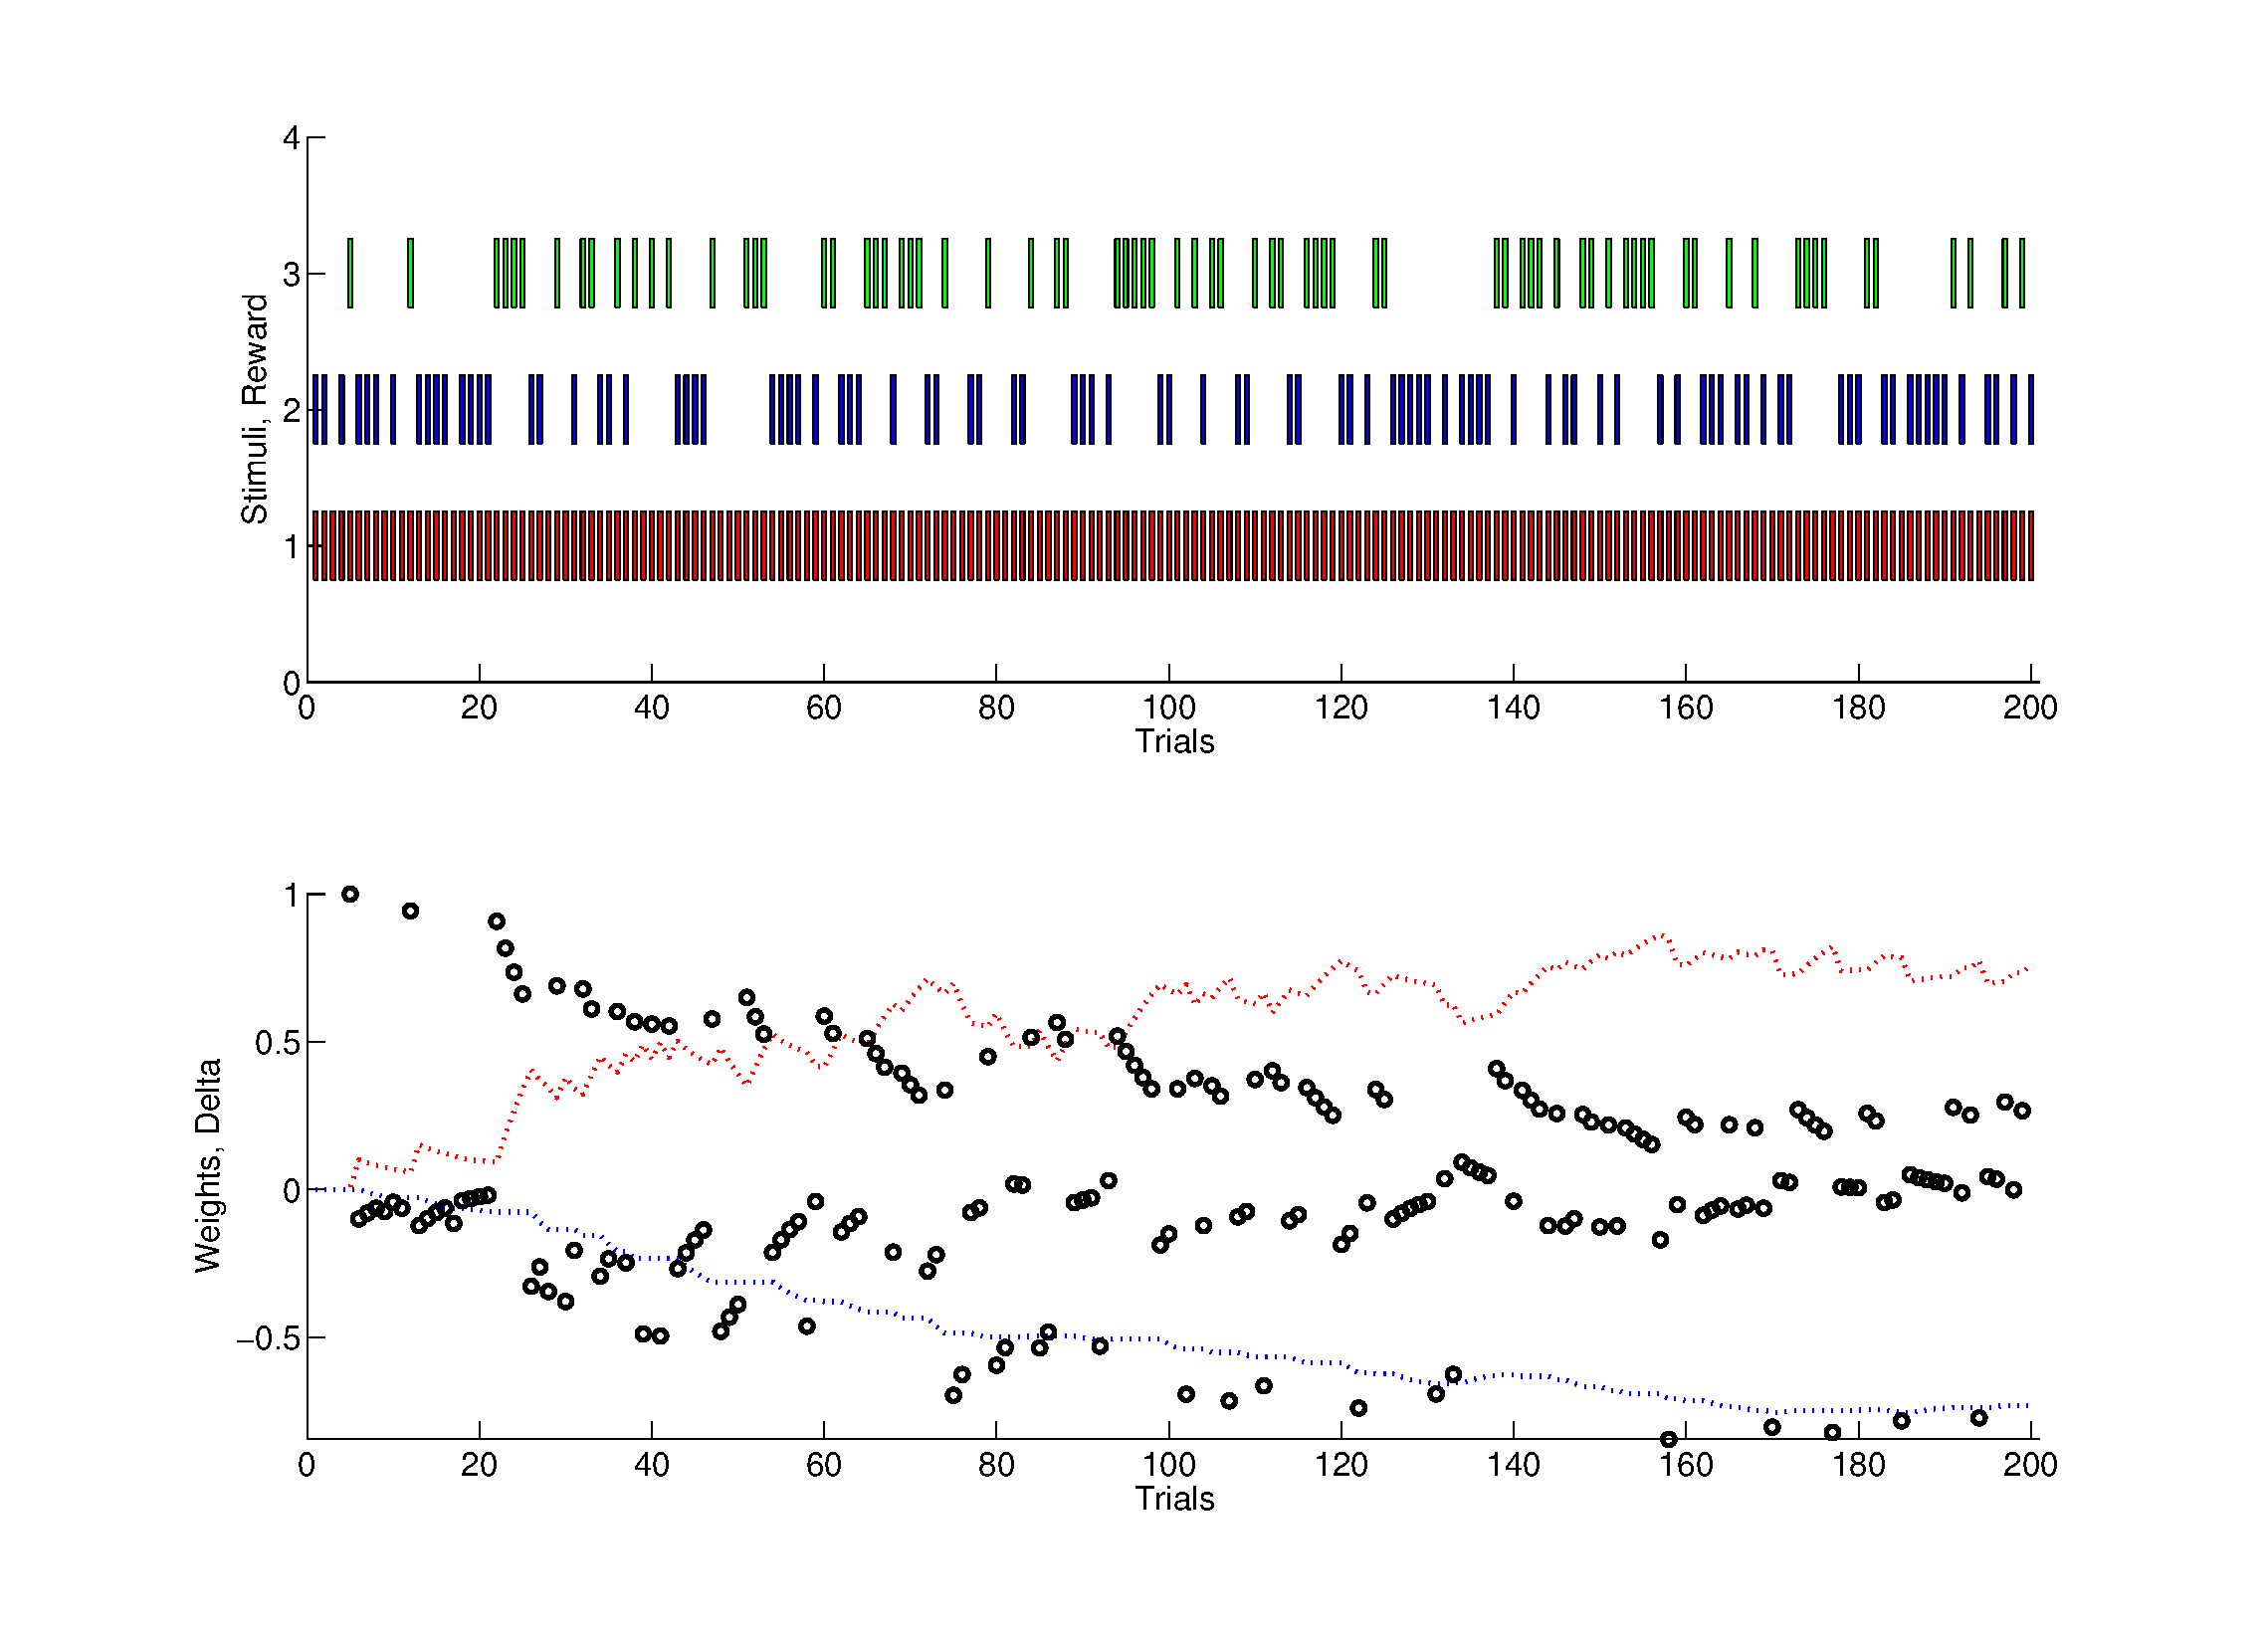
\includegraphics[width=\textwidth]{inhib.eps}
% tau4_M1.eps: 0x0 pixel, 300dpi, 0.00x0.00 cm, bb= -304   -42   918   834
\begin{footnotesize}
 Figure 2, inhibitory conditioning
\end{footnotesize}
\end{center}
\subsection{Discussion}
\begin{itemize}
\item Weights converge to the steady state values stated as $w_{ss}$, as it is seen the red dotted line converges to 3/4, and blue dotted line converges to -3/4.
\item The prediction error $\delta$ for both of the weight evolutions seem to occur more negative this time. In inhibitory conditioning, negative reward expectations form any stimulus consistently associated with the failure of an expected reward.
\end{itemize}
\section{Blocking}
This time we consider a learning scenerio with two phases.\newline
\textbf{Phase 1:}
\begin{equation*}
 p_{10}=p_{00}=1/2, \;\;\; p_{01}=p_{11}=0,\;\;\;r_{11}=r_{00}=r_{01}=0, \;\;\; r_{10}=3/4
\end{equation*}
\textbf{Phase 2:}
\begin{equation*}
 p_{11}=p_{00}=1/2, \;\;\; p_{01}=p_{10}=0,\;\;\;r_{10}=r_{10}=r_{00}=0, \;\;\; r_{11}=3/4
\end{equation*}
\begin{center}
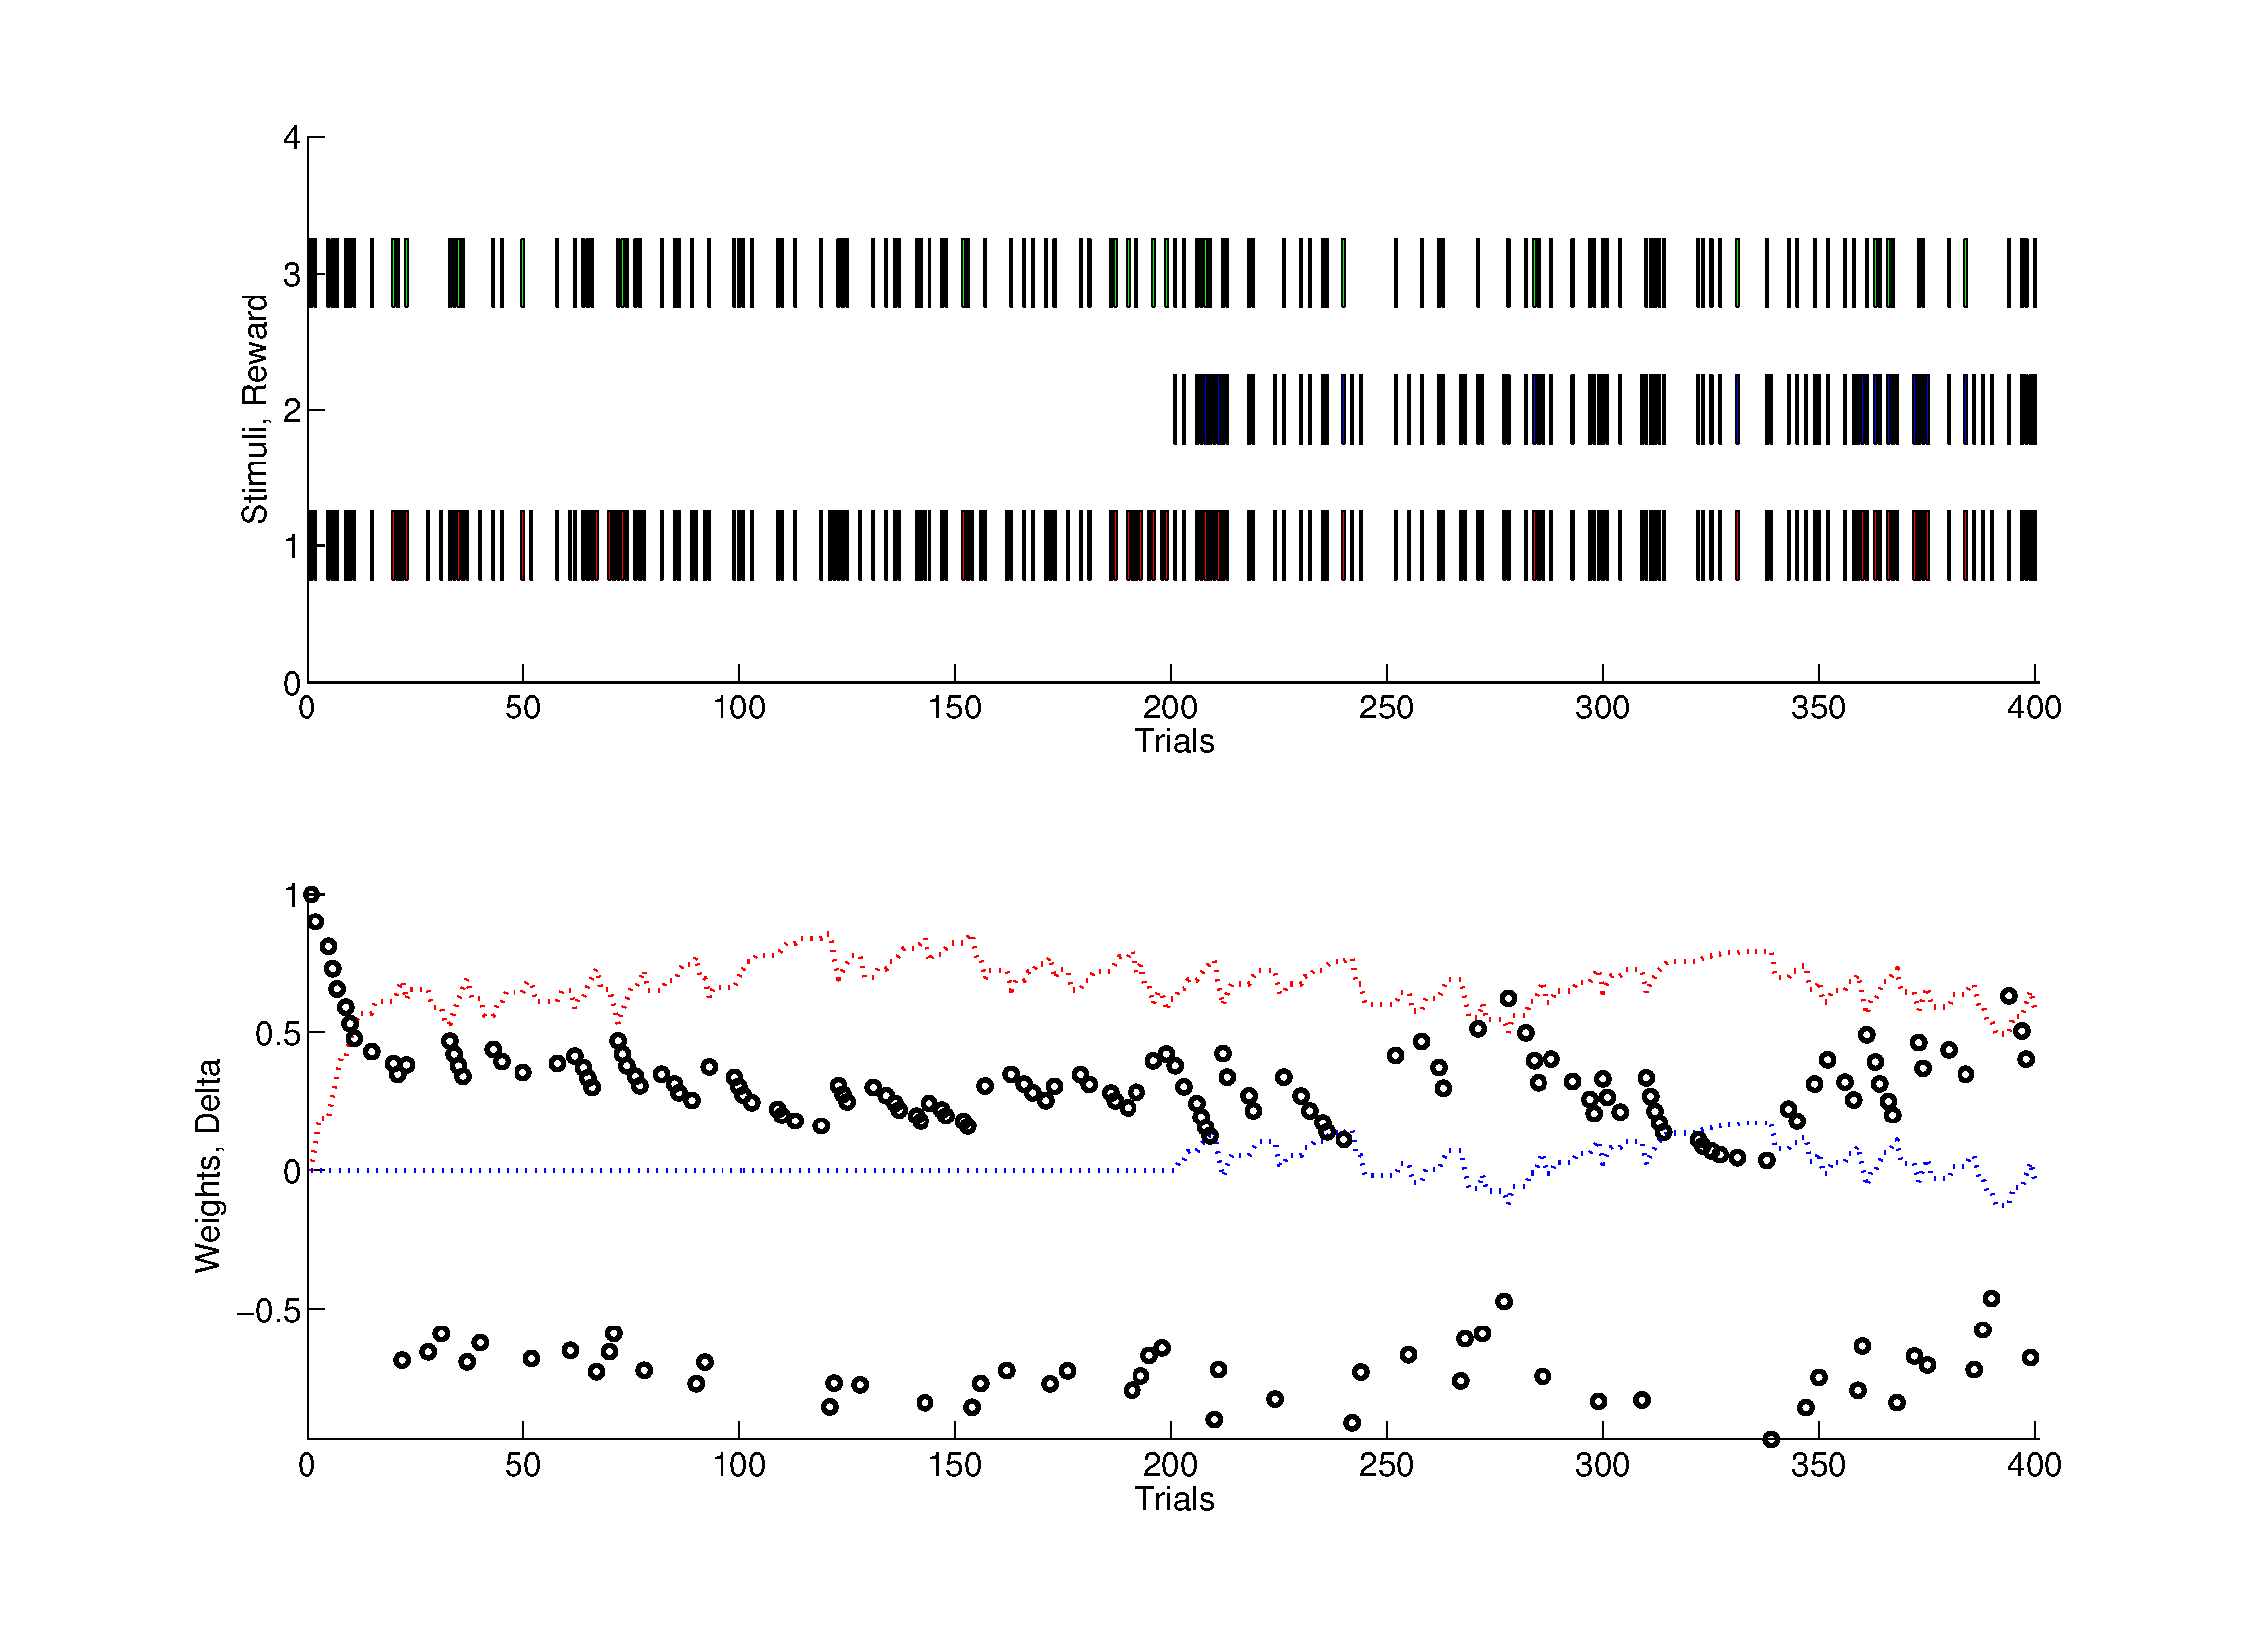
\includegraphics[width=\textwidth]{block.eps}
% tau4_M1.eps: 0x0 pixel, 300dpi, 0.00x0.00 cm, bb= -304   -42   918   834
\begin{footnotesize}
 Figure 3, blocking
\end{footnotesize}
\end{center}
\subsection{Discussion}
\begin{itemize}
\item In blocking, a previously learned reward expectation for an old stimulus blocks the formation of an association for a new stimulus which is paired with the old one.
\item 
\end{itemize}



\end{document}
